\subsection{Sensor Interaction}%
\label{sec:accelerometer-access}
%
The smartphone has a built-in MEMS accelerometer, this means that at micro-level it can measure acceleration values through capacitance changes in multiple capacitors as a result of its internal assembly (calibration mass and spring contacts) displacement. With at least a MEMS system in each plane (x,y,z), one can measure the acceleration per axis. 
\subsubsection{Sensor Data Retrieval}
\label{sec:accelerometer-data}
%
The code in listing ~\ref{lst:get_accelerometer_vals} (based on \cite{androiddevsensors}) represents the retrieval of the linear acceleration for each plane.
In the first place, the definition of the sensor type is crucial to access its values (line 9). \textbf{SensorManager} grants access to the sensors of the android device (line 7). Following, one must create a listener that checks the sensors values at a determined sampling frequency using the SensorManager's method \textbf{registerListener} (line 10). Upon doing so, one overwrites the \textbf{onSensorChanged} method (line 15) so the pretended variables that hold the values of the sensor can only be updated on smartphone movement.
An acceleration sensor measures the acceleration applied to the device but regarding the force of gravity. For this reason, the values retrieved do not represent the linear accelerations for each plane. To resolve this problem, a low pass filter can be used to isolate the force of gravity in each axis (line 28) and then remove its contibution from the acceleration values (line 33).\\
%
\lstinputlisting[language=Java,caption={Accelerometer data retrieval code},label=lst:get_accelerometer_vals,style=custom-java]{listing/accelerometerAccess.java}
%
As the control module uses both wheels tilt angle and tension applied to the motor as input, the interface with the smartphone's accelerometer wasn't enough. To generate the angles necessary and vary the tension accordingly one needs to access the phone's rotation sensors. This code is implemented in listing \ref{lst:get_rot_vals}. As the interface with the accelerometer, this latter interface needs a \textbf{SensorManager} and the creation of a listener with the \textbf{registerListener} method. Some calibrations were crucial to ensure the calculated values of the angles matched the initial smartphone position chosen. Note that percentages were used as a way to implement a control independent of the motor and wheels used. This means that using a percentage of the voltage applied and wheel tilt, one could simply use a 12V or 6V motor, for example. Therefore, the control values would be immutable. This will be tested in section \ref{sec:accelerometer-using-data-test}.\\

%
\lstinputlisting[language=Java,caption={Rotation sensor data retrieval code},label=lst:get_rot_vals,style=custom-java]{listing/rotAccess.java}
%
\subsubsection{Applying Sensor Data}
\label{sec:using-accelerometer-data}
%
The project requires that the acceleration values obtained from the sensors are applied to make the vehicle move in the intended direction with the expected speed. 
%
To implement the code referent to this sub-subsection, one must pay close attention to the axis orientation in a common device, represented in figure \ref{fig:axis-smartphone}.
%
\begin{figure}[!h]
\centering
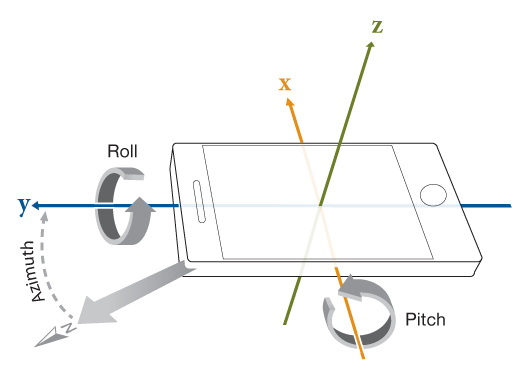
\includegraphics[width=0.85\textwidth]{img/smartphone_axis.png}
\caption{\label{fig:axis-smartphone}Axis orientation in a smartphone}
\end{figure}
%
In order to test this concept, the code presented in \ref{sec:accelerometer-data} that refers to the accelerometer was added to another project that allowed ball movement based on the accelerometer values. It must be noticed that the z acceleration value it's not relevant to the ball movement (from line 59 to 67) since only \textbf{roll} and \textbf{pitch} affect a 2D (bidimensional) object and the smartphone height relative to the ground doesn't, as one should expect by analysing figure \ref{fig:axis-smartphone}.
%
This code in listing \ref{lst:ball_mov} representing subsection \ref{sec:accelerometer-access} will be tested in \ref{sec:accelerometer-using-data-test}.\\
%
\lstinputlisting[language=Java,caption={Code for ball movement based on accelerometer data},label=lst:ball_mov,style=custom-java]{listing/ballMovement.java}
%